\documentclass[11pt]{article}
\usepackage{amssymb}
\usepackage{amsthm}
\usepackage{enumitem}
\usepackage{physics,amsmath}
\usepackage{bm}
\usepackage{adjustbox}
\usepackage{mathrsfs}
\usepackage{graphicx}
\usepackage{siunitx}
\usepackage[mathscr]{euscript}

\title{\textbf{Solved selected problems of Classical Mechanics - Gregory}}
\author{Franco Zacco}
\date{}

\addtolength{\topmargin}{-3cm}
\addtolength{\textheight}{3cm}

\newcommand{\hatr}{\bm{\hat{r}}}
\newcommand{\hatx}{\bm{\hat{x}}}
\newcommand{\haty}{\bm{\hat{y}}}
\newcommand{\hatz}{\bm{\hat{z}}}
\newcommand{\hatth}{\bm{\hat{\theta}}}
\newcommand{\hatphi}{\bm{\hat{\phi}}}
\newcommand{\hatrho}{\bm{\hat{\rho}}}
\theoremstyle{definition}
\newtheorem*{solution*}{Solution}
\renewcommand*{\proofname}{Solution}

\begin{document}
\maketitle
\thispagestyle{empty}

\section*{Chapter 10 - The linear momentum principle}

	\begin{proof}{\textbf{10.1}}
        From the linear momentum principle, we know that 
        $$\frac{dP(t)}{dt} = F(t)$$
        Then in particular, if the first state of rest happens at $t=0$ and
        the next one happens at $t=\tau$ we have that
        \begin{align*}
            \int_0^\tau dP(t) &= \int_0^\tau F(t) dt\\
            P(\tau) - P(0) &= \int_0^\tau F(t) dt
        \end{align*}
        But since they are states of rest we know that $P(\tau) = P(0) = 0$
        then
        \begin{align*}
            \int_0^\tau F(t) dt = 0 \quad\text{ so }\quad
            \frac{1}{\tau}\int_0^\tau F(t) dt = 0
        \end{align*}
        Therefore the average of the total external forces over this time
        interval is zero.

        Now let $X(t)$ be the force the sand exerts on the scale and $Mg$ be
        the force exerted on the scale by the sand and the hourglass then
        we have that
        \begin{align*}
            \frac{1}{\tau}\int_0^\tau X(t) - Mg~dt &= 0\\
            \frac{1}{\tau}\int_0^\tau X(t)dt &= Mg
        \end{align*}
        Where the first equation is equal to zero since the system goes from
        one state of rest to another and hence the time average of the apparent
        weight is the static weight $Mg$. 
    \end{proof}
\cleardoublepage
	\begin{proof}{\textbf{10.2}}
        From the linear momentum principle, we know that 
        $$\frac{dP(t)}{dt} = F(t)$$
        Let $\tau$ be the period of the system, then in particular, if
        the first rest state of the system happens at $t=0$ then the next one
        happens at $t=\tau$ so we have that
        \begin{align*}
            \int_0^\tau dP(t) &= \int_0^\tau F(t) dt\\
            P(\tau) - P(0) &= \int_0^\tau F(t) dt
        \end{align*}
        But the states between periods are rest states so we know that
        $P(\tau) = P(0) = 0$ then
        \begin{align*}
            \int_0^\tau F(t) dt = 0 \quad\text{ so }\quad
            \frac{1}{\tau}\int_0^\tau F(t) dt = 0
        \end{align*}
        Therefore the average of the total external forces over a period is
        zero.

        Now let $X(t)$ be the force the bridge exerts to the juggler (and the
        balls that are not in the air at the moment), $m$ be the mass of the
        juggler and $10M$ be the mass of all of the balls then we have that
        \begin{align*}
            \frac{1}{\tau}\int_0^\tau (X(t) - (m + 10M)g)~dt &= 0\\
            \frac{1}{\tau}\int_0^\tau X(t)dt &= (m + 10M)g
        \end{align*}
        Where the first equation is equal to zero since the system goes from
        one state of rest to another in a period. Hence the time average of
        the total force applied by the juggler to the bridge (because of the
        Third Law) is $(m + 10M)g$ which is its weight and the combined weights
        of the balls he is carrying so there is no advantage in juggling the
        balls while he crosses the bridge. 
    \end{proof}
\cleardoublepage
	\begin{proof}{\textbf{10.4}}
        Let $P$ be the linear momentum of the rope 
        \begin{align*}
            P &= \frac{M(a/2 - x/2)}{a}~v\\
                &= \frac{M(a - x)}{2a}~v
        \end{align*}
        Where we are only taking into account the free end of the rope,
        because the other end has a velocity zero. 

        Let the reaction exerted by the support at the fixed end be $R$. Then
        the total downward force is $F = Mg - R$ so we have that
        \begin{align*}
            \frac{dP}{dt} &= Mg - R\\
            \frac{d}{dt}\bigg(\frac{M(a - x)}{2a}~v\bigg) &= Mg - R\\
            \frac{M}{2a}\bigg((a - x)\frac{dv}{dt} - v^2\bigg) &= Mg - R\\
            Mg - \frac{M}{2a}\bigg((a - x)\frac{dv}{dt} - v^2\bigg) &= R
        \end{align*}
        Now replacing the value of $v$ we obtained before we have that
        \begin{align*}
            Mg - \frac{M}{2a}\bigg((a - x)\frac{2a^2 - 2ax +x^2}{2(a-x)^2}~g
            - \frac{x(2a-x)}{a-x}~g \bigg) &= R\\
            Mg - \frac{Mg}{2a}\bigg(\frac{2a^2 - 2ax +x^2}{2(a-x)}
            - \frac{x(2a-x)}{a-x} \bigg) &= R\\
            Mg - \frac{Mg}{2a}
            \bigg(\frac{2a^2 - 6ax +3x^2}{2(a-x)}\bigg) &= R\\
            Mg\bigg(1 - \frac{2a^2 - 6ax +3x^2}{4a(a-x)}\bigg) &= R\\
            \frac{Mg}{4a}\bigg(\frac{2a^2 + 2ax -3x^2}{a-x}\bigg) &= R
        \end{align*}
        Which is the reaction $R$ exerted by the support at the fixed end when
        the free end has descended a distance $x$ as we wanted.

        Now we want to find how far the free end has fallen when the reaction
        $R$ collapses at $3Mg/2$ so we want to solve for $x$ the following
        equation
        \begin{align*}
            \frac{Mg}{4a}\bigg(\frac{2a^2 + 2ax -3x^2}{a-x}\bigg) &= \frac{3Mg}{2}
        \end{align*}
        And the solutions to this equation are $x=2a/3$ and $x=2a$, but
        the second one cannot happen because $0 \leq x \leq a$.
        Therefore if the support collapses when $R$ goes beyond $3Mg/2$ at
        this moment the free end has fallen a distance $2a/3$.
    \end{proof}
\cleardoublepage
	\begin{proof}{\textbf{10.5}}
        Let $P$ be the linear momentum of the chain then
        \begin{align*}
            P &= \frac{M(a-x)}{a} v
        \end{align*}
        Where $a-x$ is the length of the chain that is still in the air when
        the chain has fallen a distance $x$.

        Let $R$ be the reaction of the table when the chain starts falling then
        the total downward force is $F = Mg - R$ so by the linear momentum
        principle we have that
        \begin{align*}
            \frac{dP}{dt} &= Mg - R\\
            \frac{d}{dt}\bigg(\frac{M(a - x)}{a}~v\bigg) &= Mg - R\\
            \frac{M}{a}\bigg((a - x)\frac{dv}{dt} - v^2\bigg) &= Mg - R
        \end{align*}
        Since the chain is falling under uniform gravity we have that
        $dv/dt = g$ which implies that $v^2 = g^2t^2$ and since $x = gt^2/2$
        we get that $v^2 = 2gx$ then
        \begin{align*}
            \frac{M}{a}\bigg((a - x)g - 2gx\bigg) &= Mg - R\\
            \frac{Mg}{a}(a - 3x) &= Mg - R\\
            3\frac{Mx}{a}g &= R
        \end{align*}
        Therefore because of the Third law the force the chain exerts to
        the table when it's falling is equal to $R$ in magnitude which implies
        that it is 3 times the weight of the chain that it's actually lying on
        the table.

        In the second case, we have that the linear momentum is given by
        \begin{align*}
            P &= \frac{Mx}{a} v
        \end{align*}
        Where $x$ is the length of the chain that has been pulled up.

        Also, the total upward force is given by
        $F=\frac{1}{3}Mg + R - Mg$ then by the linear momentum principle we
        have that
        \begin{align*}
            \frac{dP}{dt} &= \frac{1}{3}Mg + R - Mg\\
            \frac{d}{dt}\bigg(\frac{Mx}{a}~v\bigg) &= \frac{1}{3}Mg + R - Mg\\
            \frac{M}{a}\bigg(x\frac{dv}{dt} + v^2\bigg) &= \frac{1}{3}Mg + R - Mg            
        \end{align*}
        And in this case we know that $R = \frac{M(a-x)}{a}g$ which is the
        weight of chain lying on the table so we have that
        \begin{align*}
            \frac{M}{a}\bigg(x\frac{dv}{dt} + v^2\bigg)
            &= \frac{1}{3}Mg + \frac{M(a-x)}{a}g - Mg\\
            x\frac{dv}{dt} + v^2
            &= -\frac{2}{3}ag + (a-x)g\\
            x\frac{dv}{dt} + v^2
            &= \frac{1}{3}g(a -3x)
        \end{align*}
        To solve this equation let us see that $dv/dt = vdv/dx$
        and let us change variables where $w = v^2$ so $dw/dx = 2vdv/dx$
        and then
        \begin{align*}
            x\frac{dw}{dx} + 2w
            &= \frac{2}{3}g(a -3x)
        \end{align*}
        Let us also notice that
        \begin{align*}
            \frac{d(x^2w)}{dx} &= 2xw + x^2\frac{dw}{dx}\\
            \frac{1}{x}\frac{d(x^2w)}{dx} &= 2w + x\frac{dw}{dx}
        \end{align*}
        So by replacing this value we can integrate as follows
        \begin{align*}
            \frac{1}{x}\frac{d(x^2w)}{dx} &= \frac{2}{3}g(a -3x)\\
            \int d(x^2w) &= \int \frac{2}{3}g(a -3x)x dx\\
            x^2w &= \frac{2}{3}g\bigg[\frac{ax^2}{2} - x^3\bigg] + C\\
            v^2 &= \frac{1}{3}g(a - 2x) + \frac{C}{x^2}
        \end{align*}
        Where $C$ is a constant of integration.

        To determine $C$ let us assume that $v=0$ and $x=b$ when $t=0$ so we
        have that
        \begin{align*}
        0 &= \frac{1}{3}g(a - 2b) + \frac{C}{b^2}\\
        C &= -\frac{b^2}{3}g(a - 2b)
        \end{align*}
        And now if we let $b \to 0$ we see that $C = 0$. Therefore the velocity
        of the chain is given by
        \begin{align*}
            v^2 &= \frac{1}{3}g(a - 2x)
        \end{align*}
        Finally, the chain will rise to the highest height when $v=0$ and this
        will happen when $x=a/2$.   
    \end{proof}
\cleardoublepage
	\begin{proof}{\textbf{10.7}}
        We know that the Rocket equation including gravity is given by
        \begin{align*}
            m_t\frac{dv}{dt} = (-\dot{m_t})u - m_tg
        \end{align*}
        Where we named the variable mass as $m_t = m(t)$.
        given that the gravity is uniform and the ejection speed $u$ is
        constant the solution to this equation is given by
        \begin{align*}
            v(t) &= 0 + u\log\bigg(\frac{M}{m_t}\bigg) - gt\\
            v(t) &= u\log\bigg(\frac{M}{m_t}\bigg) - gt
        \end{align*}
        Where we used that $v_0 = 0$. Also, the mass function $m_t$ is given
        by
        \begin{align*}
            m_t &= -\bigg(\frac{M-m}{\tau}\bigg)t + M
        \end{align*}
        Then
        \begin{align*}
            \frac{M}{m(t)} &= \frac{M}{-(M-m)\frac{t}{\tau} + M}\\
            \frac{M}{m(t)} &= \frac{\gamma}{(1 - \gamma)\frac{t}{\tau} + \gamma}\\
            % \frac{M}{m(t)} &= \frac{\gamma\tau}{(1 - \gamma)t + \gamma\tau}\\
            \frac{M}{m(t)} &= \frac{1}{\frac{1 - \gamma}{\gamma\tau}~t + 1}
        \end{align*}
        Which implies that the velocity is given by
        \begin{align*}
            v(t) &= u\log\bigg(\frac{1}{\frac{1 - \gamma}{\gamma\tau}~t + 1}\bigg)
            - gt\\
            v(t) &= u\bigg(\log(1) -\log(\frac{1 - \gamma}{\gamma\tau}~t + 1)\bigg)
            - gt\\
            v(t) &= -u\log(\frac{1 - \gamma}{\gamma\tau}~t + 1) - gt
        \end{align*}
        Finally, the maximum speed of the rocket is achieved when all the fuel
        was burnt, which happens at $t=\tau$ then
        \begin{align*}
            v_{max} &= -u\log(\frac{1-\gamma}{\gamma} +1) - g\tau\\
            v_{max} &= u\log(\gamma) - g\tau
        \end{align*}

        To compute the height at the burnout moment let's call
        $A = \frac{1 - \gamma}{\gamma\tau}$ then
        \begin{align*}
            \frac{dz}{dt} &= -u\log(At + 1) - gt\\
            \int dz &= -u\int \log(At + 1)~dt - g \int t~dt\\
            z &= -u\bigg[\bigg(\frac{1}{A} + t\bigg)\log(At+1) - t\bigg]
            - \frac{gt^2}{2} + C
        \end{align*}
        Since $z=0$ when $t=0$ this implies that $C=0$.
        The maximum height or the height at burnout should happen at $t=\tau$
        therefore we have that
        \begin{align*}
            z &= -u\bigg[\bigg(\frac{\gamma\tau}{1-\gamma} + \tau\bigg)\log(
                \frac{1-\gamma}{\gamma}+1)- \tau\bigg] - \frac{g\tau^2}{2}\\
            z &= -u\bigg[-\bigg(\frac{\gamma\tau}{1-\gamma} + \tau\bigg)\log(\gamma)
                - \tau\bigg] - \frac{g\tau^2}{2}\\
            z &= u\bigg[\bigg(\frac{\gamma + 1 - \gamma}{1-\gamma}\bigg)\tau\log(\gamma)
                + \tau\bigg] - \frac{g\tau^2}{2}\\
            z &= u\tau\bigg(\frac{\log(\gamma)}{1-\gamma} + 1\bigg)
                - \frac{g\tau^2}{2}\\
            z &= u\tau\bigg(1 - \frac{\log(\gamma)}{\gamma-1}\bigg)
                - \frac{g\tau^2}{2}
        \end{align*}
    \end{proof}
	\begin{proof}{\textbf{10.9}}
        In this case, the Rocket Equation looks like
        \begin{align*}
            m_t\frac{dv}{dt} = (-\dot{m_t})u - \epsilon kv
        \end{align*} 
        Where we named the variable mass as $m_t = m(t)$ and also we know that
        $\dot{m_t} = -k$ and that $m_t = - kt + M$.
        Then the equation becomes
        \begin{align*}
            (M - kt)\frac{dv}{dt} &= ku - \epsilon kv\\
            \frac{dv}{dt} + \frac{\epsilon k}{M -kt}~v &= \frac{ku}{M-kt}
        \end{align*}
        Which is A First Order Linear Differential Equation and we can solve
        it as follows
        \begin{align*}
            f(t) &= e^{\int \frac{\epsilon k}{M-kt} dt}\\
            f(t) &= e^{-\epsilon\log(M-kt)}\\
            f(t) &= (M-kt)^{-\epsilon}
        \end{align*}
        Then we have that
        \begin{align*}
            v &= \frac{1}{f(t)}\int \frac{f(t)h(t)}{a(t)} dt + \frac{C}{f(t)}\\
            v &= ku(M -kt)^\epsilon \int \frac{(M -kt)^{-\epsilon}}{M -kt} dt
            + C(M -kt)^{\epsilon}\\
            v &= ku(M -kt)^\epsilon \frac{(M-kt)^{-\epsilon}}{k\epsilon}
            + C(M -kt)^{\epsilon}\\
            v &= \frac{u}{\epsilon} + C(M -kt)^{\epsilon}
        \end{align*}
        Given that $v=0$ when $t=0$ we have that
        $C = -\frac{u}{\epsilon M^\epsilon}$ so the general solution is given
        by
        \begin{align*}
            v &= \frac{u}{\epsilon}\bigg(1 -\bigg(\frac{M- kt}{M}\bigg)^{\epsilon}\bigg)
        \end{align*}
        In particular at burnout when $t=\tau$ we have that
        $m_\tau = m = -k\tau + M$ so $k = \frac{M-m}{\tau}$ then by replacing
        this and setting $\gamma = M/m$ we get that
        \begin{align*}
            V &= \frac{u}{\epsilon}\bigg(1 -\bigg(\frac{M - (M-m)}{M}\bigg)^{\epsilon}\bigg)\\
            V &= \frac{u}{\epsilon}\bigg(1 -\bigg(\frac{1}{\gamma}\bigg)^{\epsilon}\bigg)\\
            V &= \frac{u}{\epsilon}(1 -\gamma^{-\epsilon})
        \end{align*}
        Finally, we know that $\gamma^{-\epsilon} = e^{-\epsilon\log(\gamma)}$
        then the two terms approximation by Taylor series is given by
        $e^{-\epsilon\log(\gamma)} = 1 -\epsilon\log(\gamma) +
        \frac{(\epsilon\log(\gamma))^2}{2}$ so we have that
        \begin{align*}
            V &= \frac{u}{\epsilon}\bigg(1 - \bigg(1 -\epsilon\log(\gamma)
            + \frac{\epsilon^2\log(\gamma)^2}{2} + O(\epsilon^3)\bigg)\bigg)\\
            V &= u\bigg(\log(\gamma)
            - \frac{\epsilon\log(\gamma)^2}{2} + O(\epsilon^2)\bigg)\\
            V &= u\log(\gamma)\bigg(1
            - \frac{\epsilon\log(\gamma)}{2}+ O(\epsilon^2)\bigg)
        \end{align*}
    \end{proof}
\cleardoublepage
	\begin{proof}{\textbf{10.10}}
        In the first stage, given that the Rocket is in free space
        the Rocket Equation looks like this
        \begin{align*}
            m(t)\frac{dv}{dt} = -\dot{m}(t)u
        \end{align*}
        So the rocket velocity at time $t=t_1$ i.e. when we have burnout
        the fuel of the first stage is given by equation 10.9
        \begin{align*}
            v_1 = u \log(\frac{M_1 + M_2 + m_0}{\eta M_1 + M_2 + m_0})
        \end{align*}

        When we have burnout the fuel of the second stage at $t=t_2$
        the final solution to the Rocket equation in free space becomes
        \begin{align*}
            V &= v_1 + u \log(\frac{M_2 + m_0}{\eta M_2 + m_0})\\
            V &= u \log(\frac{M_1 + M_2 + m_0}{\eta M_1 + M_2 + m_0}) + 
            u \log(\frac{M_2 + m_0}{\eta M_2 + m_0})
        \end{align*}

        Now let us define $\alpha = M_2/(M_1 + M_2)$ and
        $\beta = m_0 /(M_1 + M_2)$ then 
        \begin{align*}
            V &= u \log(\frac{M_1 + M_2 + m_0}{\eta M_1 + M_2 + m_0}) + 
            u \log(\frac{M_2 + m_0}{\eta M_2 + m_0})\\
            V &= u \log(\frac{M_1 + M_2 + m_0}{\eta M_1 + M_2 + m_0} \cdot
            \frac{M_2 + m_0}{\eta M_2 + m_0})\\
            V &= u \log(
                \frac{
                    \frac{M_1 + M_2 + m_0}{M_1 + M_2}
                }{
                    \frac{\eta M_1 + M_2 + m_0}{M_1 + M_2}
                } \cdot
                \frac{
                    \frac{M_2 + m_0}{M_1 + M_2}
                }{
                    \frac{\eta M_2 + m_0}{M_1 + M_2}
                }
            )\\
            V &= u \log(
                \frac{(1 + \beta)(\alpha + \beta)}
                {(\eta - \eta\alpha + \alpha + \beta)(\eta\alpha + \beta)}
            )\\
            V &= u \log(
                \frac{(1 + \beta)(\alpha + \beta)}
                {(\eta + (1 - \eta)\alpha + \beta)(\eta\alpha + \beta)}
            )
        \end{align*}

        We are interested in maximizing $V$ and this should happen when
        $dV/d\alpha = 0$ so we compute $dV/d\alpha$ as follows
        \begin{align*}
            \frac{dV}{d\alpha} &= u~\frac{
            (\eta - 1)\eta(\alpha^2 + 2\alpha\beta -\beta)
            }{(\alpha + \beta)(-\alpha\eta + \alpha + \beta + \eta)(\alpha\eta + \beta)}
        \end{align*}
        And when $dV/d\alpha = 0$ we get that
        \begin{align*}
            \alpha^2 + 2\alpha\beta -\beta = 0
        \end{align*}
        Then this is satisfied when
        \begin{align*}
            \alpha &= \frac{-2\beta \pm\sqrt{4\beta^2 + 4\beta}}{2}\\
            \alpha &= -\beta \pm \sqrt{\beta^2 + \beta}
        \end{align*}

        Now when $\beta$ is small we have that
        \begin{align*}
            \alpha &= -\beta \pm \sqrt{\beta(1 + \beta)}\\
            \alpha &= -\beta \pm \sqrt{\beta}\bigg(1 + \frac{\beta}{2}\bigg)\\
            \alpha &= -\beta \pm \sqrt{\beta}\bigg(1 + O(\beta)\bigg)\\
            \alpha &= \pm \sqrt{\beta} + O(\beta)
        \end{align*}
        So the optimum value (approximately) of $\alpha$ is $\sqrt{\beta}$.
        Finally, replacing this value of $\alpha$ we get that
        \begin{align*}
            V &= u \log(
                \frac{(1 + \beta)(\sqrt{\beta} + \beta)}
                {(\eta + (1 - \eta)\sqrt{\beta} + \beta)(\eta\sqrt{\beta} + \beta)}
            )\\
            V &= u \log(
                \frac{(\sqrt{\beta} + \sqrt{\beta}\beta + \beta + \beta^2)}
                {(\eta + \sqrt{\beta} - \eta\sqrt{\beta} + \beta)(\eta\sqrt{\beta} + \beta)}
            )\\
            V &= u \log(
                \frac{(\sqrt{\beta} + \sqrt{\beta}\beta + \beta + \beta^2)}
                {\eta^2\sqrt{\beta} + \eta\beta - \eta^2\beta + \eta\beta\sqrt{\beta}
                + \eta\beta + \beta\sqrt{\beta} - \eta\beta\sqrt{\beta} + \beta^2
                }
            )\\
            V &= u \log(
                \frac{\sqrt{\beta} + O(\beta)}{\eta^2\sqrt{\beta} + O(\beta)}
            )\\
            V &= u \log(\frac{1}{\eta^2}) = u \log(\gamma^2)\\
            V &= 2 u \log(\gamma)            
        \end{align*}
        Where we defined $\gamma = 1/\eta$.
    \end{proof}
\cleardoublepage
	\begin{proof}{\textbf{10.13}}
        Suppose the two spheres have masses $m_1$ and $m_2$ which collide with
        initial velocities $u_1$ and $u_2$ in an elastic head-on collision,
        also, let the final velocities be $v_1$ and $v_2$.
        Since the linear momentum is conserved we have that
        \begin{align*}
            m_1u_1 + m_2u_2 &= m_1v_1 + m_2v_2\\
            m_1(u_1 - v_1) &= m_2(v_2 - u_2)\\
            m_1 &= m_2\frac{(v_2 - u_2)}{(u_1 - v_1)}
        \end{align*} 
        Also, since the energy is conserved we write the energy conservation
        equation and we replace the value of $m_1$ as follows
        \begin{align*}
            m_1u_1^2 + m_2u_2^2 &= m_1v_1^2 + m_2v_2^2\\
            m_2\frac{(v_2 - u_2)}{(u_1 - v_1)}u_1^2 + m_2u_2^2 &=
            m_2\frac{(v_2 - u_2)}{(u_1 - v_1)}v_1^2 + m_2v_2^2\\
            (v_2 - u_2)u_1^2 + (u_1 - v_1)u_2^2 &=
            (v_2 - u_2)v_1^2 + (u_1 - v_1)v_2^2\\
            (v_2 - u_2)(u_1^2 -v_1^2) &=
            (u_1 - v_1)(v_2^2 - u_2^2)\\
            (v_2 - u_2)(u_1 + v_1)(u_1 - v_1) &=
            (u_1 - v_1)(v_2 + u_2)(v_2 - u_2)\\
            u_1 + v_1 &= v_2 + u_2\\
            u_1 - u_2 &= v_2 - v_1
        \end{align*}
        Therefore we see that the relative velocity of the spheres after
        the impact is the negative of the relative velocity before the impact. 

        In the next scenario we know the collision with the floor is
        elastic but the floor doesn't move s the ball returns
        upward with the same velocity $v$.

        In the second part of the scenario, the first ball collided with the
        floor and it's returning upward with a velocity of $u_1=v$ since
        we saw the collision with the floor was elastic and the floor didn't
        move. On the other hand, the velocity of the second ball before it
        collides with the first one is $u_2 = -v$ where we assumed the
        positive direction points upward.
        After the collision, let us assume the second ball has a velocity
        $v_2 = v'$ hence using the result we derived above we have that
        $v_1 = v'- 2v$.

        Then by the conservation of linear momentum, we can derive the value
        of $v'$ in terms of $M$, $m$ and $v$ as follows 
        \begin{align*}
            Mv - m v &= M(v' - 2v) + mv'\\
            Mv - m v + 2Mv &= (M + m)v'\\
            (3M - m)v &= (M + m)v'\\
            v' &= \frac{(3M - m)}{(M + m)} v
        \end{align*}
        Finally, let $\gamma = m/M$, $v = \sqrt{2gh_t}$ and $v' = \sqrt{2gh'}$
        where $h_t$ is the height of the tube and $h'$ is the height to which
        the second ball will raise so we have that
        \begin{align*}
            \sqrt{2gh'} &= \frac{(3M - m)}{(M + m)} \sqrt{2gh_t}\\
            h' &= \frac{(3M - m)^2}{(M + m)^2} h_t\\
            h' &= \frac{9M^2 - 6Mm + m^2}{M^2 +2Mm+ m^2} h_t\\
            h' &= \frac{9 - 6\gamma + \gamma^2}{1 +2\gamma+ \gamma^2} h_t
        \end{align*}
        Now assuming $\gamma$ is small we get that
        \begin{align*}
            h' &\approx 9h_t + O(\gamma)
        \end{align*}
        Therefore the height to which the second ball will be projected is
        approximately 9 times the height of the tube. 
    \end{proof}
	\begin{proof}{\textbf{10.14}}
        From the linear momentum equation, we have that the velocity of
        the composite particle is given by 
        \begin{align*}
            (m_1 + m_2)\bm{v} &= m_1\bm{v}_1 + m_2\bm{v}_2\\
            \bm{v} &= \frac{m_1\bm{v}_1 + m_2\bm{v}_2}{m_1 + m_2}
        \end{align*}
        We also have from the energy conservation equation that $Q$,
        the kinetic energy lost as a result of the collision is given by
        \begin{align*}
            \frac{1}{2}&m_1|\bm{v}_1|^2 + \frac{1}{2}m_2|\bm{v}_2|^2
            = Q + \frac{1}{2}(m_1 + m_2)|\bm{v}|^2\\
            Q &= \frac{1}{2}m_1|\bm{v}_1|^2 + \frac{1}{2}m_2|\bm{v}_2|^2
            - \frac{|m_1\bm{v}_1 + m_2\bm{v}_2|^2}{2(m_1 + m_2)}\\
            Q &= \frac{1}{2}m_1|\bm{v}_1|^2 + \frac{1}{2}m_2|\bm{v}_2|^2
            - \frac{m_1^2|\bm{v}_1|^2 + 2m_1m_2\bm{v}_1\bm{v}_2
            + m_2^2|\bm{v}_2|^2}{2(m_1 + m_2)}\\
            Q &= \frac{1}{2}m_1|\bm{v}_1|^2 + \frac{1}{2}m_2|\bm{v}_2|^2
            - \frac{m_1^2|\bm{v}_1|^2}{2(m_1 + m_2)}
            - \frac{m_1m_2\bm{v}_1\bm{v}_2}{(m_1 + m_2)}
            - \frac{m_2^2|\bm{v}_2|^2}{2(m_1 + m_2)}\\
            Q &= \frac{1}{2}m_1\bigg[|\bm{v}_1|^2 -\frac{m_1|\bm{v}_1|^2}{m_1 + m_2}\bigg]
            + \frac{1}{2}m_2\bigg[|\bm{v}_2|^2 - \frac{m_2|\bm{v}_2|^2}{m_1 + m_2}\bigg]
            - \frac{m_1m_2\bm{v}_1\bm{v}_2}{(m_1 + m_2)}\\
            Q &= \frac{m_1m_2|\bm{v}_1|^2}{2(m_1 + m_2)}
            + \frac{m_1m_2|\bm{v}_2|^2}{2(m_1 + m_2)}
            - \frac{m_1m_2\bm{v}_1\bm{v}_2}{(m_1 + m_2)}
        \end{align*}
        Therefore the kinetic energy lost because of the collision is given by
        \begin{align*}
            Q &= \frac{m_1m_2}{2(m_1 + m_2)}|\bm{v}_1 - \bm{v}_2|^2
        \end{align*} 
    \end{proof}
\cleardoublepage
	\begin{proof}{\textbf{10.17}}
    \begin{itemize}
        \item [(i)] From equation $\bf{A}$ we have that the scattering angle
        $\theta_1$ is given by
        \begin{align*}
            \tan\theta_1 &= \frac{\sin\psi}{\cos\psi + \gamma}\\
            \theta_1 &= \arctan(\frac{\sin\psi}{\cos\psi + \gamma})
        \end{align*}
        Since $\gamma > 1$ and $0\leq \psi\leq \pi$ we have that
        $\theta_1 \geq 0$.
        The maximum value of $\theta_1$ should happen for some $\psi$ in
        the interval $0\leq \psi\leq \pi$ so we compute
        $\frac{d\theta_1}{d\psi} = 0$
        \begin{align*}
            \frac{d\theta_1}{d\psi}
            &= \frac{\gamma\cos\psi + 1}
            {\gamma^2 + 2\gamma\cos\psi + \cos^2\psi + \sin^2\psi} = 0
        \end{align*}
        And this implies that the maximum of $\theta_1$ should happen for
        \begin{align*}
            \gamma\cos\psi + 1 &= 0\\
            \psi &= \arccos(-\frac{1}{\gamma})
        \end{align*}
        Then by replacing this value, we have that
        \begin{align*}
            \tan\theta_1 &= \frac{\sin(\arccos(-\frac{1}{\gamma}))}
            {-\frac{1}{\gamma} + \gamma}\\
            \tan\theta_1 &= \frac{\sqrt{1 - (1/\gamma)^2}}
            {\frac{\gamma^2 - 1}{\gamma}}\\
            \tan\theta_1 &= \frac{\frac{\gamma^2 - 1}{\gamma^2}}
            {\frac{\sqrt{1 - (1/\gamma)^2}(\gamma^2 - 1)}{\gamma}}\\
            \tan\theta_1 &= \frac{\frac{1}{\gamma}}{\sqrt{1 - (1/\gamma)^2}}\\
            \theta_1 &=  \arcsin(\frac{1}{\gamma})
        \end{align*}
        Where we used that $\arcsin(x) = \arctan(x/\sqrt{1-x^2})$.
        Therefore we have that $0 \leq \gamma \leq \arcsin(\frac{1}{\gamma})$.
        
        \item[(ii)] From equation $\bf{C}$ we have that the opening angle is
        given by
        \begin{align*}
            \tan\theta &= \bigg(\frac{\gamma + 1}{\gamma - 1}\bigg)\cot(\frac{\psi}{2})
        \end{align*}
        If $m_1 < m_2$ then $\gamma < 1$ then $\tan\theta < 0$ and this
        implies $\pi/2 < \theta < \pi$ i.e. the opening angle is obtuse.
        
        If $m_1 > m_2$ then $\gamma > 1$ then $\tan\theta > 0$ and this
        implies $0 < \theta < \pi/2$ i.e. the opening angle is acute.
        
        \item[(iii)] From the energy conservation equation and equation $\bf{D}$
        we have that
        \begin{align*}
            E_1 &= E_0 - E_2\\
            E_1 &= E_0 - E_0 \frac{4m_1m_2}{(m_1 + m_2)^2} \sin^2(\psi/2)\\
            \frac{E_1}{E_0} &= 1 - \frac{4m_1m_2}{(m_1 + m_2)^2} \sin^2(\psi/2)\\
            \frac{E_1}{E_0} &= \frac{m_1^2 +2m_1m_2 + m_2^2 - 4m_1m_2\sin^2(\psi/2)}{(m_1 + m_2)^2}
        \end{align*}
        Since $0 \leq \sin^2(\psi/2) \leq 1$ then 
        \begin{align*}
            \frac{E_1}{E_0} &\geq \frac{m_1^2 +2m_1m_2 + m_2^2 - 4m_1m_2}{(m_1 + m_2)^2}\\
            \frac{E_1}{E_0} &\geq \frac{m_1^2 -2m_1m_2 + m_2^2}{(m_1 + m_2)^2}\\
            \frac{E_1}{E_0} &\geq \bigg(\frac{m_1 - m_2}{m_1 + m_2}\bigg)^2
        \end{align*}
        
        On the other hand, from equation $\bf{D}$ we have that
        \begin{align*}
            \frac{E_2}{E_0} &= \frac{4m_1m_2}{(m_1 + m_2)^2} \sin^2(\psi/2)
        \end{align*}
        Since $0 \leq \sin^2(\psi/2) \leq 1$ then 
        \begin{align*}
            \frac{E_2}{E_0} &\leq \frac{4m_1m_2}{(m_1 + m_2)^2}
        \end{align*}

    \end{itemize}
    \end{proof}
\cleardoublepage
	\begin{proof}{\textbf{10.18}}
        When the particles have equal mass we have that $\gamma = 1$ so the
        elastic scattering formulae becomes
        \begin{align*}
            \tan\theta_1 &= \frac{\sin\psi}{\cos\psi + 1}\\
            \tan\theta_1 &= \tan\frac{\psi}{2}\\
            \theta_1 &= \frac{\psi}{2}
        \end{align*}
        Since $\theta_2$ doesn't depend on $\gamma$ it doesn't change
        \begin{align*}
            \theta_2 = \frac{1}{2}(\pi - \psi)
        \end{align*}
        We know that $\tan\theta$ is given by
        \begin{align*}
            \tan\theta = \bigg(\frac{\gamma + 1}{\gamma -1}\bigg)\cot(\psi / 2)
        \end{align*}
        So when $\gamma = 1$ we have that $\tan\theta \to \infty$ which implies
        that $\theta = \frac{\pi}{2}$.\\
        For $E_2/E_0$ we have that
        \begin{align*}
            \frac{E_2}{E_0} &= \frac{4\gamma}{(\gamma + 1)^2}\sin^2(\psi/2)\\
            \frac{E_2}{E_0} &= \frac{4}{2^2}\sin^2(\psi/2)\\
            \frac{E_2}{E_0} &= \sin^2(\psi/2)
        \end{align*}
        And for $E_1/E_0$ we use the energy conservation equation where
        $E_1 + E_2 = E_0$ then
        \begin{align*}
            \frac{E_1}{E_0} &= 1 - \frac{E_2}{E_0}\\
            \frac{E_1}{E_0} &= 1 - \sin^2(\psi/2)\\
            \frac{E_1}{E_0} &= \cos^2(\psi/2)
        \end{align*}

        Now we want to know at which angle the experimenter should look to find
        neutrons of energy $E/4$ then by using the equation relating $E_1$ and $E_0$
        we compute the ZM scattering angle as follows
        \begin{align*}
            \cos^2(\psi/2) &= \frac{E/4}{E}\\
            \cos^2(\psi/2) &= \frac{1}{4}
        \end{align*}
        This implies that $\psi/2 = 60^\circ$ i.e. $\psi = 120^\circ$.
        The scattering angle is given by $\theta_1 = \psi/2$ and hence
        $\theta_1 = 60^\circ$. Therefore to see scattered neutrons with energy
        $E/4$ we must look at an angle of $60^\circ$.\\
        But if the recoil neutrons are the ones that have $E/4$ energy then
        using the equation relating $E_2$ and $E_0$ we compute the ZM
        scattering angle as follows
        \begin{align*}
            \sin^2(\psi/2) &= \frac{E/4}{E}\\
            \sin^2(\psi/2) &= \frac{1}{4}
        \end{align*}
        This implies that $\psi/2 = 30^\circ$ i.e. $\psi = 60^\circ$.
        The recoil angle is then given by $\theta_2 = 1/2(\pi - \psi)$ and
        hence $\theta_2 = 60^\circ$. Therefore to see recoil neutrons with
        energy $E/4$ we must look at the same angle of $60^\circ$.\\
        This implies that there are no other energies we can see at the same
        angle.
    \end{proof}
\cleardoublepage
	\begin{proof}{\textbf{10.20}}
        Let $m_1$ and $m_2$ be the masses of the visible and non-visible
        components of the binary star Cygnus X-1. 
        Also, let $a_1$ and $a_2$ be the semi-major axes of the orbits
        of each component respectively. By positioning the origin in the
        center of mass of the system the equation for the center of mass
        becomes
        \begin{align*}
            -m_2a_2 &= m_1a_1\\
            a_2 &= -\frac{m_1a_1}{m_2}
        \end{align*}
        Also, we know that $a = a_1 + a_2$ where $a$ is the semi-major axis of
        the relative orbit. Then we have that
        \begin{align*}
            a &= \bigg(1 + \frac{m_1}{m_2}\bigg)a_1
        \end{align*}
        Now replacing this value in the equation (10.26) for the period we get
        that
        \begin{align*}
            \tau^2 &= \frac{4\pi^2(m_2 + m_1)^3a_1^3}{G(m_1 + m_2)m_2^3}\\
            m_2^3G\tau^2 &= 4\pi^2(m_2 + m_1)^2a_1^3\\
            \frac{m_2^3G\tau^2}{4\pi^2a_1^3} &= m_2^2 + 2m_2m_1 + m_1^2\\
            \frac{m_2^3G\tau^2}{4\pi^2a_1^3} - m_2^2 - 2m_2m_1 &- m_1^2 = 0
        \end{align*}
        In terms of astronomical units (where $G=4\pi^2$ and $5.6$ days are
        0.015 years) this gives
        \begin{align*}
            \frac{m_2^3(0.015)^2}{(0.09)^3} - m_2^2 - 40m_2 &- 400 = 0            
        \end{align*}
        By solving this cubic equation we get that the only real solution
        for the non-visible component is $16.41 M_{\odot}$.
    \end{proof}
\cleardoublepage
	\begin{proof}{\textbf{10.23}}
    The system described looks like the following    
    \begin{center}
        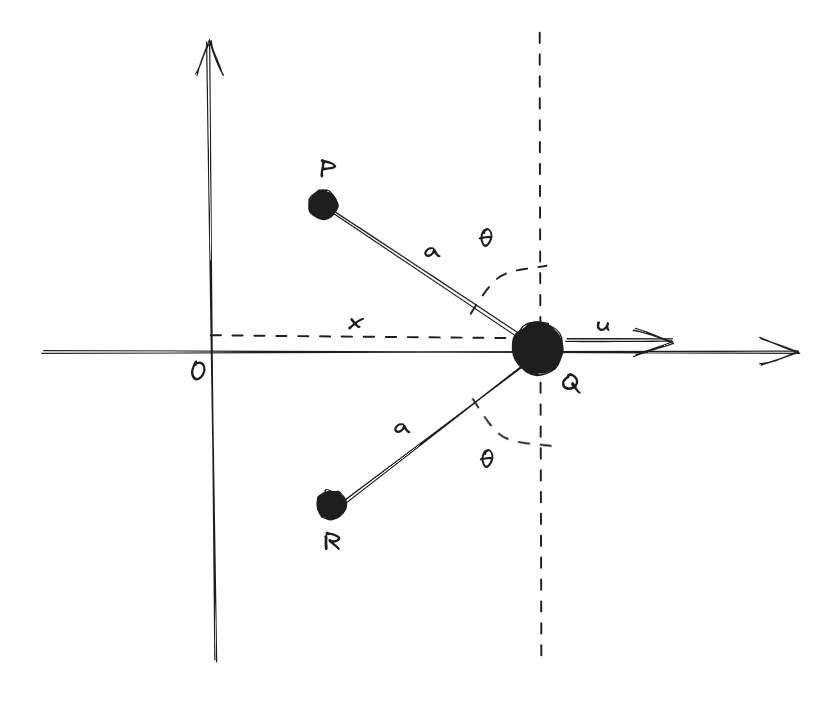
\includegraphics[scale=0.4]{ch10-23.png}
    \end{center}
    Also, the velocity diagrams look like
    \begin{center}
        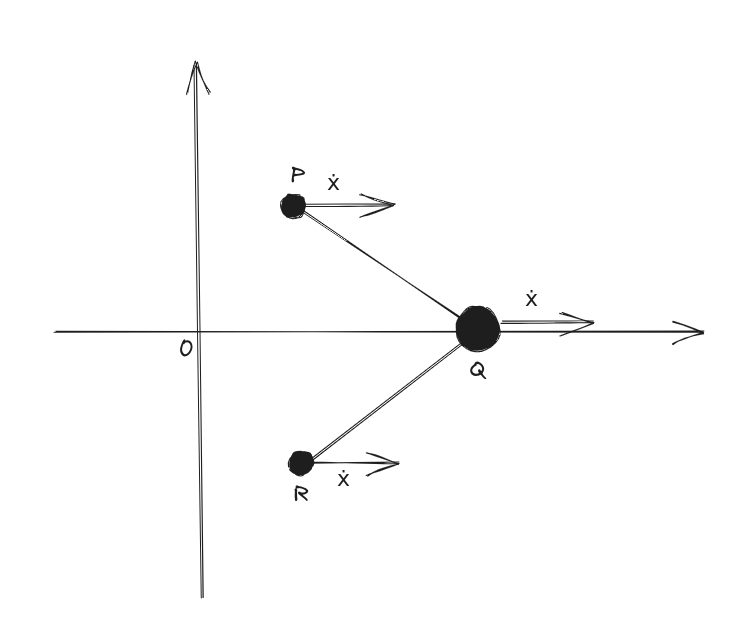
\includegraphics[scale=0.3]{ch10-23-1.png}
        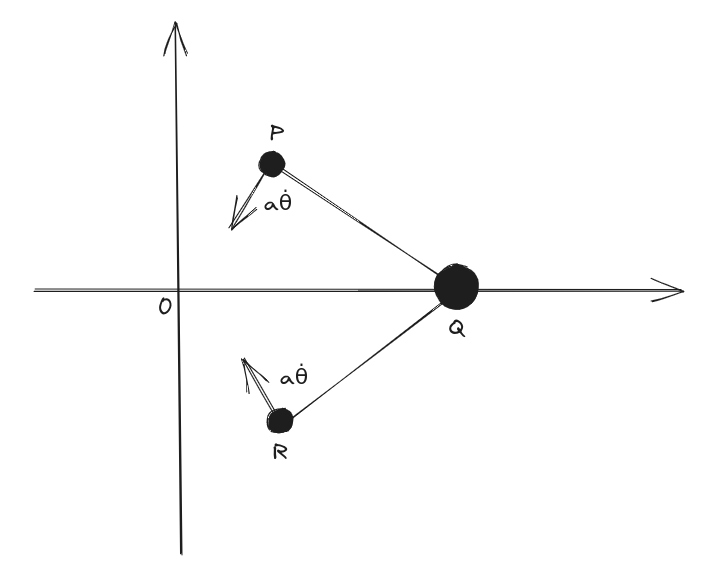
\includegraphics[scale=0.3]{ch10-23-2.png}
    \end{center}
    Since the horizontal table is smooth, there are no external forces in
    the system then the horizontal component of the linear momentum is
    conserved so from the velocity diagram we have that
    \begin{align*}
        P_h = 2m\dot{x} + 2m(\dot{x} - a\dot{\theta}\cos(\theta)) = C
    \end{align*}
    Where the horizontal component for $a\dot{\theta}$ is
    $a\dot\theta\cos(\theta)$ but it is augmenting opposite to $\dot x$ so
    we take the negative.
    From the initial conditions, we know that $C = 2mu$ hence
    \begin{align*}
        2m\dot{x} + 2m(\dot{x} - a\dot{\theta}\cos(\theta)) &= 2mu\\
        2\dot{x} - a\dot{\theta}\cos(\theta) &= u
    \end{align*}

    Since the horizontal table is smooth, there are no constraint forces
    exerted and the tensions in the inextensible strings do no work in total
    then the energy is conserved.
    
    From the velocity diagram, the kinetic energy of the system at
    time $t$ is given by
    \begin{align*}
        T &= \frac{1}{2}(2m)\dot x^2 +
        \frac{1}{2}(2m)(\bm{\dot x} + \bm{a \dot\theta})^2\\
        T &= m\dot x^2 +
        m(\dot x^2 + (a\dot\theta)^2 - 2 \dot x (a\dot\theta) \cos(\theta))
    \end{align*}
    Where $\bm{\dot x}$ and $\bm{a \dot\theta}$ are the velocity vectors.

    There are no contributions to the gravitational potential energy and
    taking into account the initial conditions we have that
    \begin{align*}
        m\dot x^2 +
        m(\dot x^2 + (a\dot\theta)^2 - 2 \dot x (a\dot\theta) \cos(\theta))
        &= mu^2\\
        2\dot x^2 + (a\dot\theta)^2 - 2 \dot x (a\dot\theta) \cos(\theta))
        &= u^2
    \end{align*}
    So by replacing the value of $2\dot x$ from the first equation into
    the second one we get that
    \begin{align*}
        \frac{(u + a\dot{\theta}\cos(\theta))^2}{2} + (a\dot\theta)^2
        - (u + a\dot{\theta}\cos(\theta))(a\dot\theta) \cos(\theta)
        &= u^2\\
        \frac{u^2}{2} + ua\dot{\theta}\cos(\theta)
        + \frac{(a\dot{\theta})^2\cos^2(\theta)}{2}
        + (a\dot\theta)^2 - \quad&\\
        - [u(a\dot\theta) \cos(\theta) + (a\dot\theta)^2 \cos^2(\theta)]
        &= u^2\\
        (a\dot\theta)^2 - \frac{(a\dot{\theta})^2\cos^2(\theta)}{2}
        &= \frac{u^2}{2}\\
        (a\dot\theta)^2( 2 - \cos^2(\theta))
        &= u^2\\
        \dot{\theta}^2 &= \frac{u^2}{a^2}\bigg(\frac{1}{2 - \cos^2(\theta)}\bigg)
    \end{align*}
    Finally, to determine the time $t$ when P and R will collide we can solve
    this differential equation as follows
    \begin{align*}
        \frac{u}{a} &= \sqrt{2 - \cos^2(\theta)}~\frac{d\theta}{dt}\\
        \frac{u}{a} \int_0^t dt &= \int_0^{\pi/2} \sqrt{2 - \cos^2(\theta)}~d\theta\\
        t &= \frac{a}{u}\int_0^{\pi/2} \sqrt{2 - \cos^2(\theta)}~d\theta
    \end{align*}
    Where we used as integral limit $\pi/2$ since they will collide when
    $\theta$ reaches this value.
    \end{proof}
\cleardoublepage
	\begin{proof}{\textbf{10.24}}
    The system described looks like this
    \begin{center}
        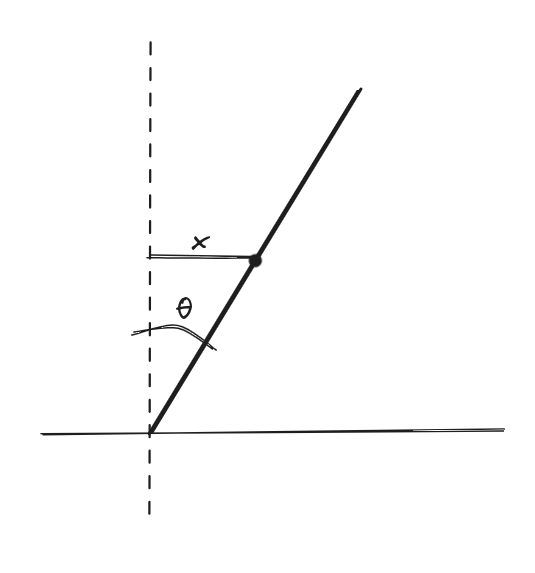
\includegraphics[scale=0.5]{ch10-24.png}
    \end{center}
    Also, the velocity diagram looks like
    \begin{center}
        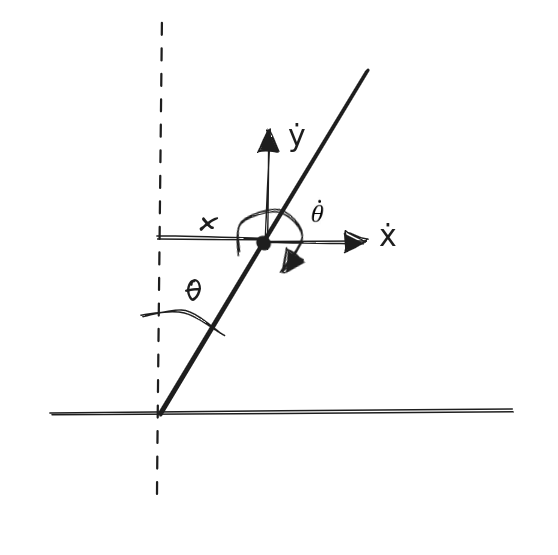
\includegraphics[scale=0.5]{ch10-24-1.png}
    \end{center}
    Since the horizontal table is smooth, there are no external forces in
    the system then the horizontal component of the linear momentum is
    conserved so from the velocity diagram we have that
    \begin{align*}
        P_x = M\dot{x} = C
    \end{align*}
    From the initial conditions, we see that $\dot{x} = 0$ which implies that
    the center of mass of the rod moves in a vertical straight line.

    Now the kinetic energy of the system at time $t$ is given by
    \begin{align*}
        T &= \frac{1}{2}M\dot{y}^2
        + \frac{1}{2}\bigg(\frac{1}{3}Ma^2\bigg)\dot{\theta}^2\\
        T &= \frac{1}{2}M(-a\dot\theta\sin\theta)^2 
        + \frac{1}{2}\bigg(\frac{1}{3}Ma^2\bigg)\dot{\theta}^2\\
        T &= \frac{1}{2}Ma^2\dot\theta^2\sin^2\theta
        + \frac{1}{6}Ma^2\dot{\theta}^2
    \end{align*}
    Since we have gravitational potential energy contributions then
    the potential energy is given by
    \begin{align*}
        V = Mga\cos\theta 
    \end{align*}
    Since the system was released from rest with $\theta = 60^\circ$, the
    initial value of T is zero, while the initial value of
    $V = \frac{1}{2}Mga$. Hence, the conservation of energy implies that
    \begin{align*}
        \frac{1}{2}Ma^2\dot\theta^2\sin^2\theta + \frac{1}{6}Ma^2\dot{\theta}^2
        + Mga\cos\theta &= \frac{1}{2}Mga\\
        \frac{1}{2}a\dot\theta^2\sin^2\theta + \frac{1}{6}a\dot{\theta}^2
        + g\cos\theta &= \frac{g}{2}\\
        \frac{a\dot\theta^2}{3}(3\sin^2\theta + 1)
        &= g(1 - 2\cos\theta)\\
        \dot\theta^2
        &= \frac{3g}{a}\frac{1 - 2\cos\theta}{4 -3\cos^2\theta}
    \end{align*}
    
    Finally, the rod will hit the table when $\theta = \pi/2$ so we need to
    solve the above differential equation to find the time $t$ it takes the
    rod to hit the table
    \begin{align*}
        \frac{3g}{a}\frac{1 - 2\cos\theta}{4 -3\cos^2\theta}
        &= \bigg(\frac{d\theta}{dt}\bigg)^2\\
        \int_0^t\sqrt{\frac{3g}{a}}dt
        &= \int_{\pi/3}^{\pi/2}\sqrt{\frac{4 -3\cos^2\theta}{1 - 2\cos\theta}}d\theta\\
        t &= \sqrt{\frac{a}{3g}}
        \int_{\pi/3}^{\pi/2}\sqrt{\frac{4 -3\cos^2\theta}{1 - 2\cos\theta}}d\theta\\
        t &= 1.178 \sqrt{\frac{a}{g}}
    \end{align*}
    \end{proof}

\end{document}






















